

\documentclass[a4paper,12pt,spanish]{article}

\usepackage[utf8]{inputenc}


\usepackage{blindtext}
%\usepackage{microtype}
\usepackage{amsfonts, amsmath, amsthm, amssymb}
%\usepackage{fancyhdr}
%\usepackage{index}
%\usepackage{multicol}    

\usepackage[T1]{fontenc}
\usepackage[utf8]{inputenc}
\usepackage{graphicx}
\usepackage[spanish,es-tabla]{babel}
\usepackage{url}
\usepackage{enumitem}

\usepackage[unicode=true, pdfusetitle,
bookmarks=true,bookmarksnumbered=false,bookmarksopen=false,
breaklinks=true,pdfborder={0 0 1},backref=false,colorlinks=false]
{hyperref}

\usepackage{listings}


\usepackage{siunitx} %para el sistema internacional
\usepackage[export]{adjustbox}
\usepackage{booktabs} 
\usepackage{subcaption}

\usepackage{float}


\newcommand{\address}[1]{
	\par {\raggedright #1
		\vspace{1.4em}
		\noindent\par}
}


\pagenumbering{gobble}
\include{noNumberPage}
\pagenumbering{arabic}
\setcounter{page}{48}

%tutorial de tablas latex: https://manualdelatex.com/tutoriales/tablas

\usepackage{multirow}

% \usepackage[table,xcdraw]{xcolor}


%Inicio del documento (hasta que se cierre con \end{document}
\begin{document}
	
	
	\title{Circuitos lineales RC y RL: comportamiento transitorio}
	
	%\author{Adrián Rivero Fernández}
	\date{}
	
	\maketitle
	
	
	
	\begin{abstract} %resumen
		
		Estudiaremos el comportamiento transitorio de circuitos RC y RL. Determinaremos sus constantes de tiempo e inferiremos los valores de capacidad o autoinducción utilizados.
		
	\end{abstract}

\section{Introducción}


\begin{table}[H]
	\begin{minipage}[t]{.48\linewidth}
		
		\begin{figure}[H]
			\centering
			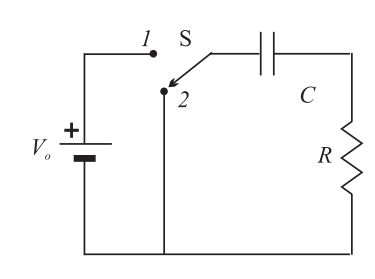
\includegraphics[width=1\linewidth]{RC}
			\caption{Circuito RC}
			\label{fig:rc}
		\end{figure}
		
	\end{minipage}\hfill
	\mbox{}
	\begin{minipage}[t]{.48\linewidth}% -----------------------tabla 2
		
		
		\begin{figure}[H]
			\centering
			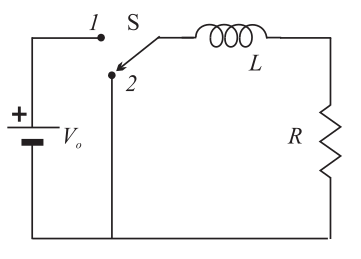
\includegraphics[width=1\linewidth]{RL}
			\caption{Circuito RL}
			\label{fig:rl}
		\end{figure}
		
	\end{minipage}\hfill
	\mbox{}
\end{table}




 

El comportamiento transistorio en un circuito RC o RL se produce al ser sometido el circuito a voltaje en forma de escalón.

La ecuación diferencial para la aplicación de este tipo de voltaje se obtiene a partir de la ley de Kirchhoff:
\begin{itemize}
	\item{Circuito RC:\\
		\[V_o = R\cdot i + \frac{q}{C} = R \cdot i + \frac{1}{C}\int i dt\]}
	\item{Circuito RL:\\
	\[V_o = R\cdot i + L \frac{di}{dt}\]}
\end{itemize}

En caso de cortocircuito, se pondrá $V_o = 0$. Y obtendremos la corriente que circula resolviendo las ecuaciones con $i=\frac{dq}{dt}$.

\subsection*{Circuito RC (conexión)}

Las condiciones iniciales son $t= 0$, $q= 0$, $i = V_o/R$, la carga máxima es la carga para $t= \infty$: $Q_o = C \cdot V_o $:

\[ q= Q_o \left(1 - \exp\left( -\frac{t}{RC} \right)\right)\]
\[i = \frac{V_o}{R} \exp\left( -\frac{t}{RC} \right)\]

Vemos que la intensidad que circula por el circuito durante la carga decae a 1/e para un tiempo $t= RC = \tau$. 

Este tiempo se llama constante de tiempo o tiempo de relajación, y nos da idea de la rapidez con la que se carga el condensador.

\subsection*{Circuito RL (conexión)}

Condiciones iniciales $t= 0$, $i = 0$:
\[ i= \frac{V_o}{R}\left[1 - \exp\left(-\frac{R}{L}t\right)\right] \]


\subsection*{Circuito RC (cortocircuito)}

Condiciones iniciales: $t= 0$, $q= Q_o = CV_o$, de modo que:
\[q = Q_o \exp\left(-\frac{t}{RC}\right)\]
\[i = - \frac{V_o}{R} \exp \left(- \frac{t}{RC}\right)\]

\subsection*{Circuito RL (cortocircuito)}

Condiciones iniciales: $t= 0$, $i= I_o = V_o/R$
\[i = \frac{V_o}{R}\exp\left(-\frac{R}{L}t\right)\]

La constante de tiempo es $\tau = L/R$

\section{Material y Métodos}

Utilizaremos un osciloscopio de doble canal, un generador de funciones, con opcion de onda cuadrada, un potenciómetro de 10$\si{k\ohm}$, dos condensadores de $0,5 \si{\micro F}$ y $0,3 \si{\micro F}$ y dos autoinducciones de $0,3 \si{H}$ y $0,15 \si{H}$.


\begin{figure}[H]
	\centering
	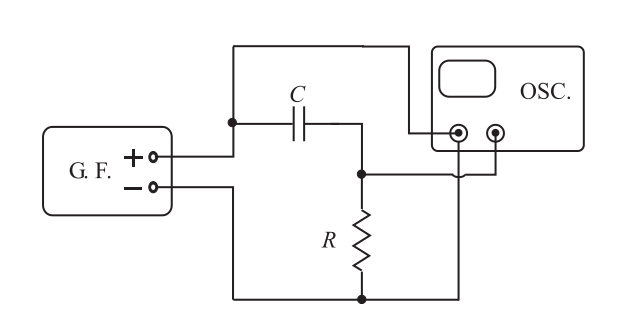
\includegraphics[width=0.9\linewidth]{montaje}
	\caption{Montaje del circuito}
	\label{fig:montaje}
\end{figure}

\subsection*{Circuito RC}

Disponemos los aparatos como inica la figura 3, aplicamos el generador de funciones como fuente de voltaje en forma de onda rectangular o cuadrada, de modo que su periodo sea mucho mayor que la constante de tiempo del circuito, calculándola previamente.

Ajustamos el osciloscopio para visualizar el voltaje en bornes de R y medimos el intervalo de tiempos $\tau$.

Repetiremos esto para distintos valores de R, teniendo cuidado de que mantengamos la forma exponencial de la curva, ya que con resistencias elevadas no se visualiza bien la carga y descarga del condensador.

Realizaremos las mediciones con ambos condensadores.


\subsection*{Circuito RL}

Repetiremos lo anterior cambiando el condensador por una autoinducción L. Mediremos para distintos valores de L.



\section{Resultados y discusión}

\subsection*{Circuito RC}

Los resultados obtenidos para $\tau$ están representados, para el primer condensador, en la Tabla 1 y la Figura 4, y para el segundo condensador en la Tabla 2 y Figura 5.

\begin{table}[H]
	\centering
	\begin{tabular}{|llll|}
		\hline
		\multicolumn{4}{|c|}{Condensador 1: $C = 0,5\pm 0,1 \si{\micro F}$}                                                       \\ \hline
		\multicolumn{1}{|l|}{R ($\si{\ohm}$)}    & \multicolumn{1}{l|}{$\tau_{teorico}$ (s)} & \multicolumn{1}{l|}{$V_o$ (V)} & $\tau_{exp.} $ (s) \\ \hline
		\multicolumn{1}{|l|}{2000$\pm100$} & \multicolumn{1}{l|}{0,001$\pm 0,0003$}       & \multicolumn{1}{l|}{2,7$\pm 0,1$}   & 0,001$\pm 0,0001$            \\ \hline
		\multicolumn{1}{|l|}{2500$\pm100$} & \multicolumn{1}{l|}{0,0013$\pm 0,0003$}     & \multicolumn{1}{l|}{2,7$\pm 0,1$}   & 0,0014 $\pm 0,0001$          \\ \hline
		\multicolumn{1}{|l|}{3000$\pm100$} & \multicolumn{1}{l|}{0,0015$\pm 0,0004$}      & \multicolumn{1}{l|}{2,7$\pm 0,1$}   & 0,0016 $\pm 0,0001$          \\ \hline
		\multicolumn{1}{|l|}{3500$\pm100$} & \multicolumn{1}{l|}{0,0018$\pm 0,0004$}     & \multicolumn{1}{l|}{2,7$\pm 0,1$}   & 0,0018    $\pm 0,0001$       \\ \hline
		\multicolumn{4}{|c|}{Pendiente: $m = 0,52 \cdot 10^{-6}$}                                               \\ \hline
	\end{tabular}
	\caption{resultados para condensador 1}
\end{table}

\begin{figure}[H]
	\centering
	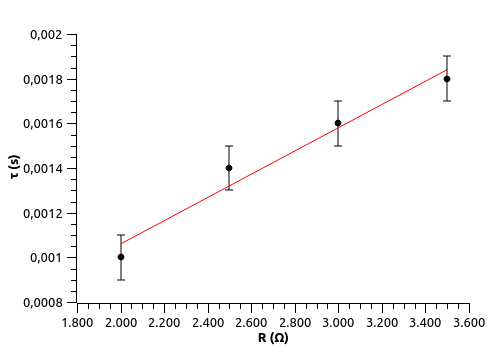
\includegraphics[width=0.8\linewidth]{RC1}
	\caption{Tiempo en función de R para el condensador 1}
	\label{fig:rc1}
\end{figure}



\begin{table}[H]
	\centering
	\begin{tabular}{|llll|}
		\hline
		\multicolumn{4}{|c|}{Condensador 2: $C = 0,3\pm 0,1 \si{\micro F}$}                                                       \\ \hline
		\multicolumn{1}{|l|}{R ($\si{\ohm}$)}    & \multicolumn{1}{l|}{$\tau_{teorico}$ (s)} & \multicolumn{1}{l|}{$V_o$ (V)} & $\tau_{exp.}$ (s) \\ \hline
		\multicolumn{1}{|l|}{1000$\pm100$} & \multicolumn{1}{l|}{0,0003$\pm 0,0001$}      & \multicolumn{1}{l|}{2,7$\pm 0,1$}   & 0,0004$\pm 0,0001$           \\ \hline
		\multicolumn{1}{|l|}{2000$\pm100$} & \multicolumn{1}{l|}{0,0006$\pm 0,0002$}      & \multicolumn{1}{l|}{2,7$\pm 0,1$}   & 0,0008$\pm 0,0001$           \\ \hline
		\multicolumn{1}{|l|}{3000$\pm100$} & \multicolumn{1}{l|}{0,0009$\pm 0,0003$}      & \multicolumn{1}{l|}{2,7$\pm 0,1$}   & 0,0012$\pm 0,0001$           \\ \hline
		\multicolumn{1}{|l|}{4000$\pm100$} & \multicolumn{1}{l|}{0,0012$\pm 0,0004$}      & \multicolumn{1}{l|}{2,7$\pm 0,1$}   & 0,0014 $\pm 0,0001$          \\ \hline
		\multicolumn{4}{|c|}{Pendiente: $m = 0,34 \cdot 10^{-6}$}                                               \\ \hline
	\end{tabular}
	\caption{resultados para condensador 2}
	\label{tab:my-table}
\end{table}

\begin{figure}[H]
	\centering
	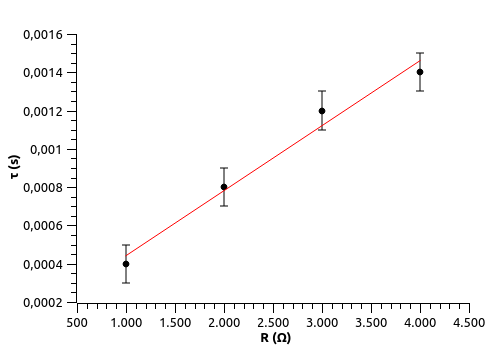
\includegraphics[width=0.8\linewidth]{RC2}
	\caption{Tiempo en función de R para el condensador 2}
	\label{fig:rc2}
\end{figure}




\subsection*{Circuito RL}

De igual forma, se presentan los resultados en la Tabla 3 y Figura 6 para la bobina 1, y en la Tabla 4 y Figura 7 para la bobina 2.

\begin{table}[H]
	\centering
	\begin{tabular}{|llll|}
		\hline
		\multicolumn{4}{|c|}{Bobina 1: L = 0,3$\pm0,01$ H}                                                                     \\ \hline
\multicolumn{1}{|l|}{R ($\si{\ohm}$)}    & \multicolumn{1}{l|}{$\tau_{teorico}$ (s)} & \multicolumn{1}{l|}{$V_o$ (V)} & $\tau_{exp.}$ (s) \\ \hline
		\multicolumn{1}{|l|}{400$\pm100$}  & \multicolumn{1}{l|}{0,0008$\pm 0,0002$}     & \multicolumn{1}{l|}{3$\pm 0,1$}     & 0,0008$\pm 0,0001$        \\ \hline
		\multicolumn{1}{|l|}{500$\pm100$}  & \multicolumn{1}{l|}{0,0006$\pm 0,00014$}      & \multicolumn{1}{l|}{3,2$\pm 0,1$}   & 0,0005$\pm 0,0001$           \\ \hline
		\multicolumn{1}{|l|}{1000$\pm100$} & \multicolumn{1}{l|}{0,0003$\pm 0,00004$}      & \multicolumn{1}{l|}{3,3$\pm 0,1$}   & 0,0002$\pm 0,0001$           \\ \hline
		\multicolumn{1}{|l|}{1500$\pm100$} & \multicolumn{1}{l|}{0,0002$\pm 0,00002$}      & \multicolumn{1}{l|}{3,8$\pm 0,1$}   & 0,0001$\pm 0,0001$           \\ \hline
		\multicolumn{4}{|c|}{Pendiente $ m = 0.36$}                                               \\ \hline
	\end{tabular}
	\caption{resultados para la bobina 1}
	\label{tab:my-table}
\end{table}



\begin{figure}[H]
	\centering
	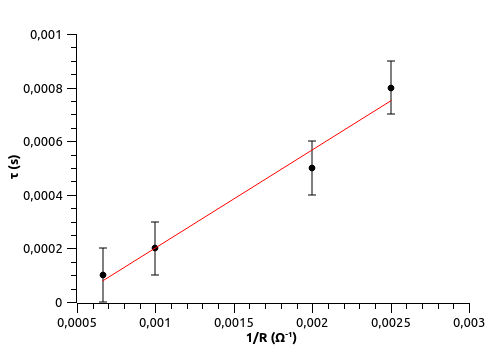
\includegraphics[width=0.8\linewidth]{RL1}
	\caption{Tiempo en función de 1/R para la bobina 1}
	\label{fig:rl1}
\end{figure}

\begin{table}[H]
	\centering
	\begin{tabular}{|llll|}
		\hline
		\multicolumn{4}{|c|}{Bobina 1: L = 0,15$\pm0,01$ H}                                                                    \\ \hline
\multicolumn{1}{|l|}{R ($\si{\ohm}$)}    & \multicolumn{1}{l|}{$\tau_{teorico}$ (s)} & \multicolumn{1}{l|}{$V_o$ (V)} & $\tau_{exp.}$ (s) \\ \hline
		\multicolumn{1}{|l|}{300$\pm100$} & \multicolumn{1}{l|}{0,0005$\pm0,0002$}      & \multicolumn{1}{l|}{2,7$\pm 0,1$}   & 0,0005$\pm 0,0001$           \\ \hline
		\multicolumn{1}{|l|}{400$\pm100$} & \multicolumn{1}{l|}{0,00038$\pm0,00012$}    & \multicolumn{1}{l|}{3$\pm 0,1$}     & 0,0004$\pm 0,0001$           \\ \hline
		\multicolumn{1}{|l|}{500$\pm100$} & \multicolumn{1}{l|}{0,0003$\pm0,00008$}      & \multicolumn{1}{l|}{3,4$\pm 0,1$}   & 0,0003$\pm 0,0001$           \\ \hline
		\multicolumn{1}{|l|}{600$\pm100$} & \multicolumn{1}{l|}{0,00025$\pm0,00006$}     & \multicolumn{1}{l|}{3,5$\pm 0,1$}   & 0,0002$\pm 0,0001$           \\ \hline
		\multicolumn{4}{|c|}{Pendiente $m = 0.17$}                                                \\ \hline
	\end{tabular}
	\caption{resultados para la bobina 2}
	\label{tab:my-table}
\end{table}





\begin{figure}[H]
	\centering
	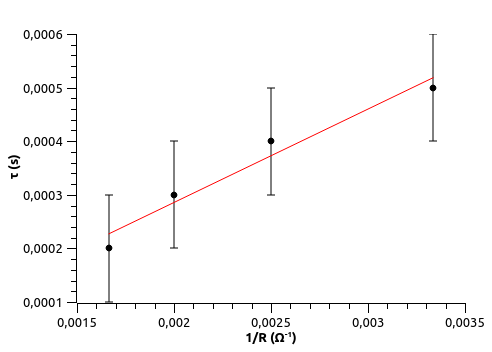
\includegraphics[width=0.8\linewidth]{RL2}
	\caption{Tiempo en función de 1/R para la bobina 2}
	\label{fig:rl2}
\end{figure}


\subsection*{Conclusión}

Hemos visto como los tiempos mantienen una relación con la resistencia en los circuitos RC y con la inversa de la resistencia en los RL. Se comprueba que la pendiente de la recta que ajusta esa relación coincide con el valor del condensador o la bobina empleada.


%%%%%%%%%%%%%%%%%%%%%%%%%%%
\begin{thebibliography}{3}
	%%%%%%%%%%%%%%%%%%%%%%%%%%%
	
	
	\bibitem{UNED2022} (varios) Guiones de prácticas- Técnicas Experimentales II. Grado en Física. Versión 2.1  UNED, 2022 \url{https://2022.cursosvirtuales.uned.es/o/3754218}
%	\bibitem{UNED2021} (varios) Técnicas Experimentales I. Versión 3.5.  UNED, 2021 \url{https://2021.cursosvirtuales.uned.es/o/42035617}
	%\bibitem{2021} Densidad de materiales \url{ https://www.stemm.com/index.php/es/densidades-de-materiales }
	
	
\end{thebibliography}


\end{document}

